% !TEX program = xelatex
\documentclass[aspectratio=169]{beamer}
\usepackage[italian]{babel}
\usepackage{animate}
\usepackage{mathtools,color}
\usepackage[makeroom]{cancel}
\usepackage{multicol}
\usepackage{mathrsfs}
\usepackage{tikz}
\usepackage{fontspec}
\usepackage{booktabs}
%\usepackage{bbold}
\usepackage[bold-style=ISO]{unicode-math}
\setmainfont{XITS}
\setmathfont{XITS Math}
\setmathfont[range={\mathcal,\mathbfcal},StylisticSet=1]{XITS Math}


\usetikzlibrary{fadings}
\usetikzlibrary{patterns}
\usetikzlibrary{shadows.blur}
\usetikzlibrary{shapes}


\usetheme{Rochester}

\definecolor{codegreen}{rgb}{0,0.6,0}
\definecolor{codegray}{rgb}{0.5,0.5,0.5}
\definecolor{codepurple}{rgb}{0.58,0,0.82}
\definecolor{backcolour}{rgb}{0.95,0.95,0.92}
 
\newfontfamily\Lato[Ligatures=TeX]{Lato}

\usefonttheme{professionalfonts}

\setsansfont{Lato}[
  UprightFont=*-Light,
  ItalicFont=*-LightItalic,
  BoldFont=*-Regular,
  BoldItalicFont=*-Italic
]

\renewcommand{\CancelColor}{\color{red}}



\uselanguage{Italian}
\languagepath{Italian}



\title{Transfer learning per selezionare gli informative-frame in una laringoscopia usando learned features}
\subtitle{Tesi di Laurea in Ingegneria Informatica}
\date{A.A. 2020/2021}
\author{Laureando: Bortolin Simone\\Relatore: Nanni Loris} 
\begin{document}

\begin{frame}
    \maketitle
\end{frame}

\begin{frame}
            \tableofcontents
\end{frame}

\section{Transfer Learning}
\begin{frame}{Transfer Learning}
    \begin{figure}[ht]
        \centering
        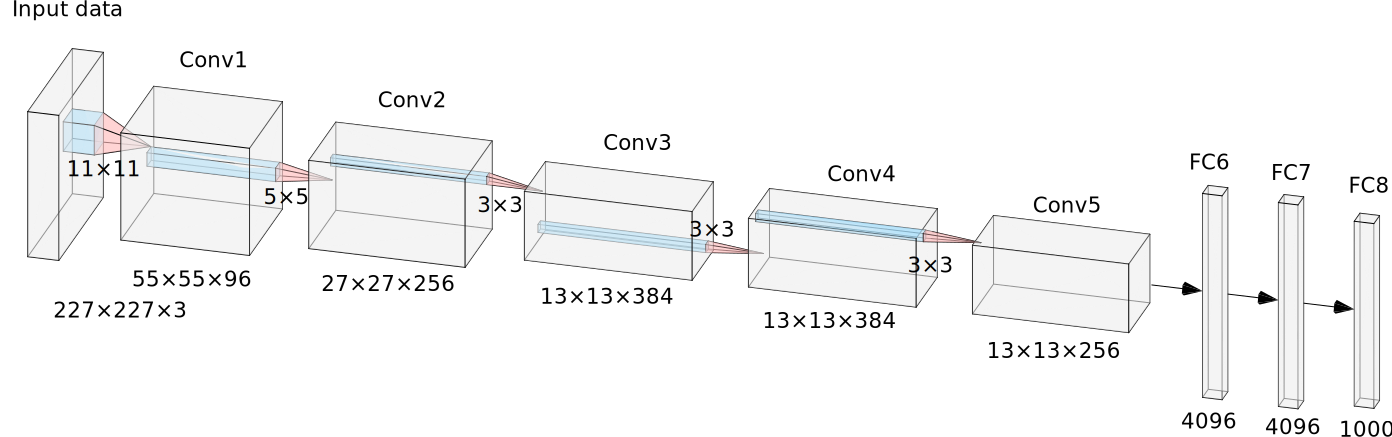
\includegraphics[width=0.5\textwidth]{addestramento-rete-neurale/alexnet.pdf}
        \caption{Architettura della CNN AlexNet}
        \label{fig:alexnet}
    \end{figure}
    \begin{figure}[ht]
        \centering
        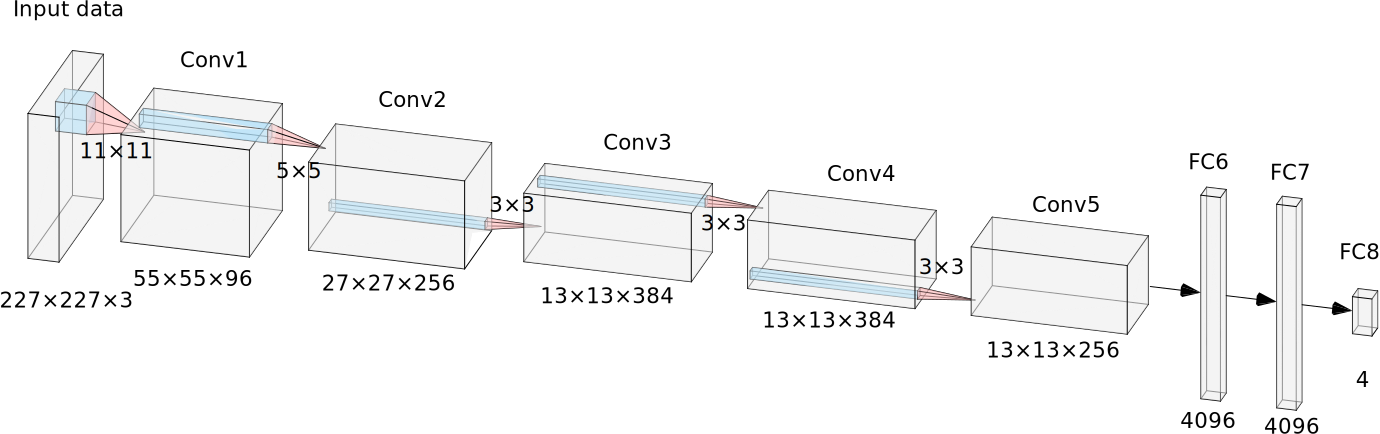
\includegraphics[width=0.5\textwidth]{addestramento-rete-neurale/alexnet-tl.pdf}
        \caption{Architettura della rete neurale AlexNet adeguata alla classificazione del dataset oggetto di studio}
        \label{fig:alexnet-tl}
    \end{figure}
\end{frame}

\begin{frame}{Transfer Learning}{Two Round turing}
    
\begin{figure}[ht]
    \centering
    \includegraphics[width=0.6\textwidth]{transfer-learning/tl_2rt.pdf}
    \caption[Schema dei due approcci: In giallo il One round turing (1R), in verde il Two round tuning]{Schema dei due approcci: In giallo il One round turing (1R), in verde il Two round tuning. Le frecce piene denotano l'input per l'addestramento, le frecce tratteggiate denotano i flussi di output (modelli addestrati).}
    \label{fig:tl_2rt}
\end{figure}
\end{frame}

\section{Preprocessing}
\begin{frame}{Preprocessing}
    
\end{frame}

\section{Data augmentation}
\begin{frame}{Data augmentation}
    
\end{frame}

\begin{frame}{Data augmentation}{Discrete cousene transform}
    
\end{frame}

\section{Risultati}
\begin{frame}{Risultati}
    \begin{table}[H]
        \centering
        \begin{tabular}{l|cc|cc}
                                         & \multicolumn{2}{c|}{1R}                                                   & \multicolumn{2}{c}{2R}                                                   \\
                                         & (1) & (2) & (1) & (2) \\ \midrule
        Semplice DA                      & 95.4\%                            & 100\%                                & 97.5\%                            & 100\%                                \\
        Filtro Contrasto Semplice        & 96.2\%                            & 100\%                                & 96.2\%                            & 100\%                                \\
        Filtro Contrasto con media e STD & 89.6\%                            & 91.7\%                               & 92.9\%                            & 100\%                                \\
        CLAHE                            & 63.7\%                            & 45.8\%                               &                                   &                                      \\
        Correzione Gamma                 & 95.0\%                            & 100\%                                &                                   &                                      \\
        Correzione Gamma e CLAHE         & 46.0\%                            & 0\%                                  &                                   &                                      \\
        Noise                            & 96.7\%                            & 100\%                                & 95.4\%                            & 95.0\%                               \\
        DCT e Noise                      & 94.6\%                            & 100\%                                & 93.8\%                            & 100\%                             
        \end{tabular}
        \caption[Specchio riassuntivo delle performance singole dei vari metodi analizzati]{Specchio riassuntivo delle performance singole dei vari metodi analizzati, (1): Divisione corretta nelle 4 classi, (2): Riconoscimento dei frame Informative}
        \label{tab:specchio-single}
    \end{table}
\end{frame}

\end{document}